\documentclass[a4paper,12pt]{article}
\usepackage{amsmath}
\usepackage{amssymb}
\usepackage[utf8]{inputenc}
\usepackage[T1]{fontenc}
\usepackage{lmodern}
\usepackage{indentfirst}
\usepackage{geometry}
\usepackage{array}
\usepackage[pdftex]{color,graphicx}
\usepackage{subfigure}
\usepackage{afterpage}
\usepackage{setspace}
\usepackage{color}
\usepackage{wrapfig}
\usepackage{listings} 
\usepackage{datetime}
\usepackage{epstopdf}
\usepackage{hyperref}

\renewcommand{\onehalfspacing}{\setstretch{1.6}}

\geometry{tmargin=2.5cm,bmargin=2.5cm,lmargin=2.5cm,rmargin=2.5cm}
\setlength{\parindent}{1cm}
\setlength{\parskip}{0mm}

\newenvironment{lista}{
\begin{itemize}
  \setlength{\itemsep}{1pt}
  \setlength{\parskip}{0pt}
  \setlength{\parsep}{0pt}
}{\end{itemize}}

\newcommand{\linia}{\rule{\linewidth}{0.4mm}}

\definecolor{lbcolor}{rgb}{0.95,0.95,0.95}
\lstset{
  backgroundcolor=\color{lbcolor},
  tabsize=4,
  language=C++,
  captionpos=b,
  tabsize=3,
  frame=lines,
  numbers=left,
  numberstyle=\tiny,
  numbersep=5pt,
  breaklines=true,
  showstringspaces=false,
  basicstyle=\footnotesize,
  identifierstyle=\color{magenta},
  keywordstyle=\color[rgb]{0,0,1},
  commentstyle=\color{green},
  stringstyle=\color{red}
  }

\begin{document}

\noindent
\begin{tabular}{|c|p{11cm}|c|} \hline 
Michał Szczygieł & Aleksander Śmierciak & \ddmmyyyydate\today \tabularnewline
\hline 
\end{tabular}


\section*{Zadanie 5 - Mnożenie macierzy na GPU}

Programem spełniającym polecenie zadania 5. jest taki, który wykona mnożenie dwóch macierzy kwadratowych przy użyciu karty graficznej, np. za pomocą CUDA.
\\

\begin{lstlisting}
    dim3 dimBlock;
    dimBlock.x = matrixSize;
    dimBlock.y = matrixSize;

    float *hostA = initializeMatrix(matrixSize);
    float *hostB = initializeMatrix(matrixSize);

    int allocBuffer = matrixSize * matrixSize * sizeof(float);
    float *devA = allocateDeviceMemory(allocBuffer);
    float *devB = allocateDeviceMemory(allocBuffer);
    float *devC = allocateDeviceMemory(allocBuffer);

    copyHostMemoryToDevice(hostA, devA, allocBuffer);
    copyHostMemoryToDevice(hostB, devB, allocBuffer);

    cudaEvent_t start, stop;
    createTimerEvents(start, stop);

    startTimer(start);

    matrixMultiplyKernel<<<dimBlock, threadCount>>>(devA, devB, devC, matrixSize);

    stopTimer(stop);

    cout << readExecutionTime(start, stop) << endl;

    destroyTimerEvents(start, stop);
    freeMemory(devA, hostA, devB, hostB, devC);
\end{lstlisting}


Etapy wykonania programu wykorzystującego CUDA można wydzielić następująco:
\begin{enumerate}
\item Ustawienie zmiennej typu struktury dim3, która przechowuje informacje o wymiarach problemu z zadania.
\item Zainicjalizowanie macierzy wejściowych, używając generatora liczb pseudo-losowych.
\item Zainicjalizowanie macierzy wejściowych przesłanych do jądra CUDA.
\item Transfer danych do macierzy jądra CUDA.
\item Wykonanie mnożenia macierzy, opatrzone zdarzeniami startu i stopu pomiaru czasu.
\item Zwolnienie pamięci.
\end{enumerate}


\section*{Przebieg}
Aby wykonać wykresy opisane w poleceniu należało również napisać program mnożący dwie macierze przy użyciu procesora centralnego.
Taki program, korzystający z dyrektyw OpenMP, pozwolił na utworzone poniższego wykresu kolumnowego: \\
\begin{center}
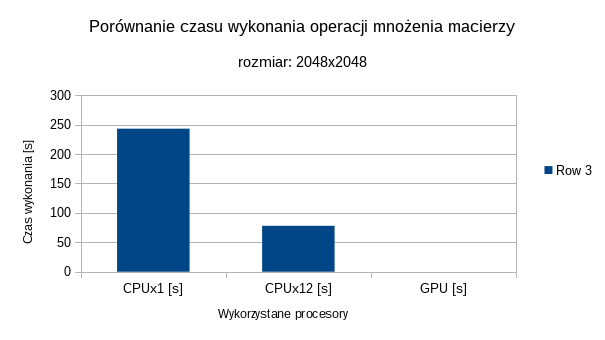
\includegraphics[width=0.7\textwidth]{data/wykonanie.png}
\end{center}

Przy tworzeniu takiego programu nie wykonano żadnych optymalizacji; implementacja jest „naiwnym” mnożeniem odpowiadających komórek macierzy.
\\
Program mnożący dwie macierze przy użyciu karty graficznej pozwolił odnotować czasy wykonania rzędu 0.003 sekundy – liczba rzędów wielkości, o jakie wydajność płynąca z użycia procesora karty graficznej przewyższa wydajność płynącą z użycia procesora centralnego jest niesamowita.\\


\end{document}